\documentclass{beamer}
\usepackage[utf8]{inputenc}
\usepackage{graphicx}
\usepackage{hyperref}

\title{Network Intrusion Detection Using XGBoost on CIC-IDS2017 Dataset}
\author{Sangay Thinley}
\institute{School of Built Environment, Engineering and Computing\\ Leeds Beckett University}
\date{\today}

\begin{document}

\frame{\titlepage}

% Slide 1: Introduction
\begin{frame}{Introduction}
\begin{itemize}
    \item Focus: Develop an efficient NIDS using classical ML.
    \item Dataset: CIC-IDS2017 – realistic network traffic with benign and multiple attack types.
    \item Goal: Accurate multi-class intrusion detection with computational efficiency.
\end{itemize}
\end{frame}

% Slide 2: Dataset Overview
\begin{frame}{Dataset Overview: CIC-IDS2017}
\begin{itemize}
    \item 2.8M network flows, 78 features, 15 attack types.
    \item Classes include: DDoS, Botnet, PortScan, Heartbleed, Infiltration, Web attacks.
    \item Raw data required cleaning, encoding, scaling, and handling of missing values.
\end{itemize}
\end{frame}

% Slide 3: Data Preprocessing
\begin{frame}{Data Preprocessing}
\begin{itemize}
    \item Missing values imputed with column mean.
    \item Categorical features: One-Hot Encoding (protocol) and Label Encoding (labels).
    \item Feature scaling: StandardScaler (mean=0, std=1).
    \item Class imbalance handled with SMOTETomek and XGBoost scale\_pos\_weight.
\end{itemize}
\end{frame}

% Slide 4: Model Selection
\begin{frame}{Model Selection: XGBoost}
\begin{itemize}
    \item Chosen for efficiency, scalability, and performance on tabular data.
    \item Gradient boosting ensemble of decision trees with L1/L2 regularization.
    \item Handles missing values and supports parallel processing.
\end{itemize}
\end{frame}

% Slide 5: Experimental Setup
\begin{frame}{Experimental Setup}
\begin{itemize}
    \item Train/Test split: 70/30 with stratified sampling.
    \item Metrics: Accuracy, Precision, Recall, F1-score, ROC-AUC, False Positive Rate.
    \item Hyperparameter tuning: Randomized + Grid Search with 5-fold CV.
\end{itemize}
\end{frame}

% Slide 6: Hyperparameter Tuning
\begin{frame}{Hyperparameter Tuning}
\begin{itemize}
    \item Optimized parameters: deeper trees, lower learning rate, more estimators.
    \item Result: Improved performance vs baseline (default hyperparameters).
    \item Balanced high F1-Macro across all attack classes.
\end{itemize}
\end{frame}

% Slide 7: Optimized Model Performance
\begin{frame}{Optimized XGBoost Performance}
\begin{itemize}
    \item High True Positive Rate; low False Positive/Negative Rate.
    \item F1-Macro: 0.98; strong detection of rare attacks (e.g., Heartbleed, Infiltration).
    \item Feature importance: Flow Packets, Flow Duration, Total Length of Fwd Packets.
\end{itemize}
\begin{figure}
    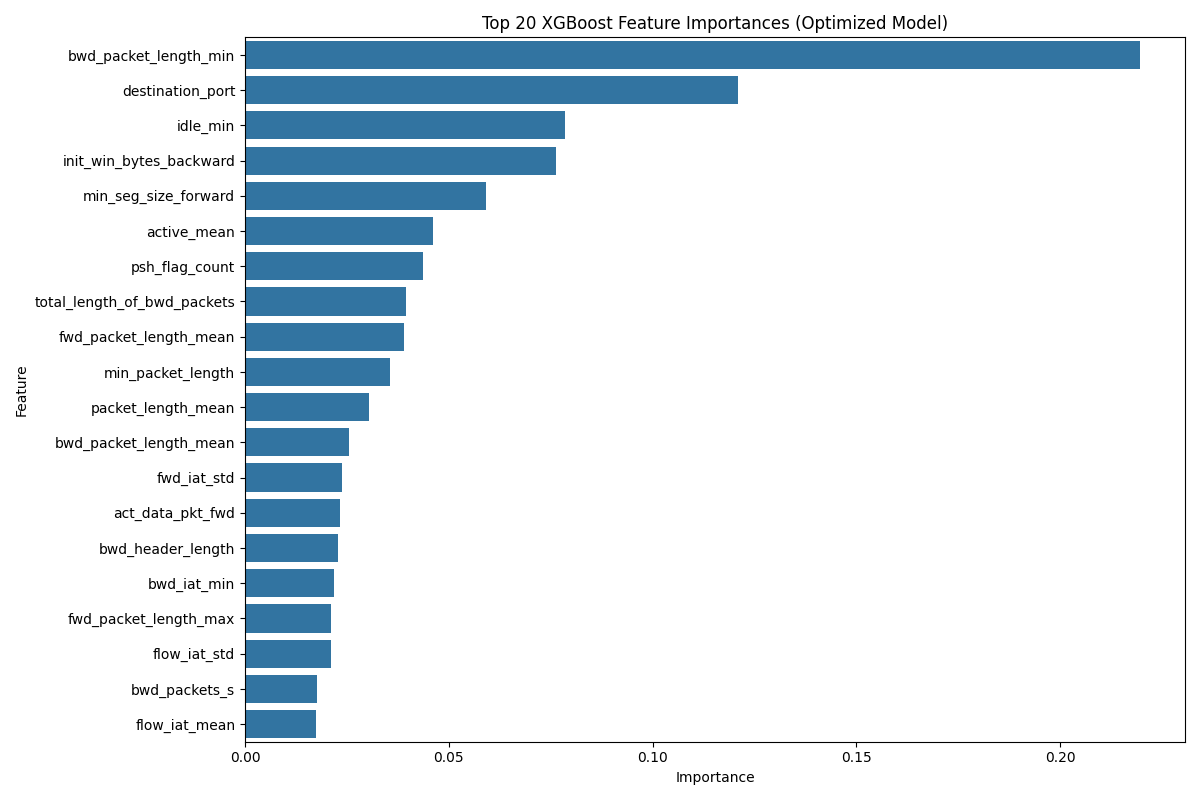
\includegraphics[width=0.7\linewidth]{assets/figures/results/xgboost_feature_importance.png}
    \caption{Top Features by XGBoost Importance}
\end{figure}
\end{frame}

% Slide 8: SHAP Analysis
\begin{frame}{SHAP Feature Impact}
\begin{itemize}
    \item Visualizes contribution of each feature to model predictions.
    \item High values of Flow Packets/s push predictions towards DDoS class.
    \item Confirms model uses relevant network flow characteristics.
\end{itemize}
\begin{figure}
    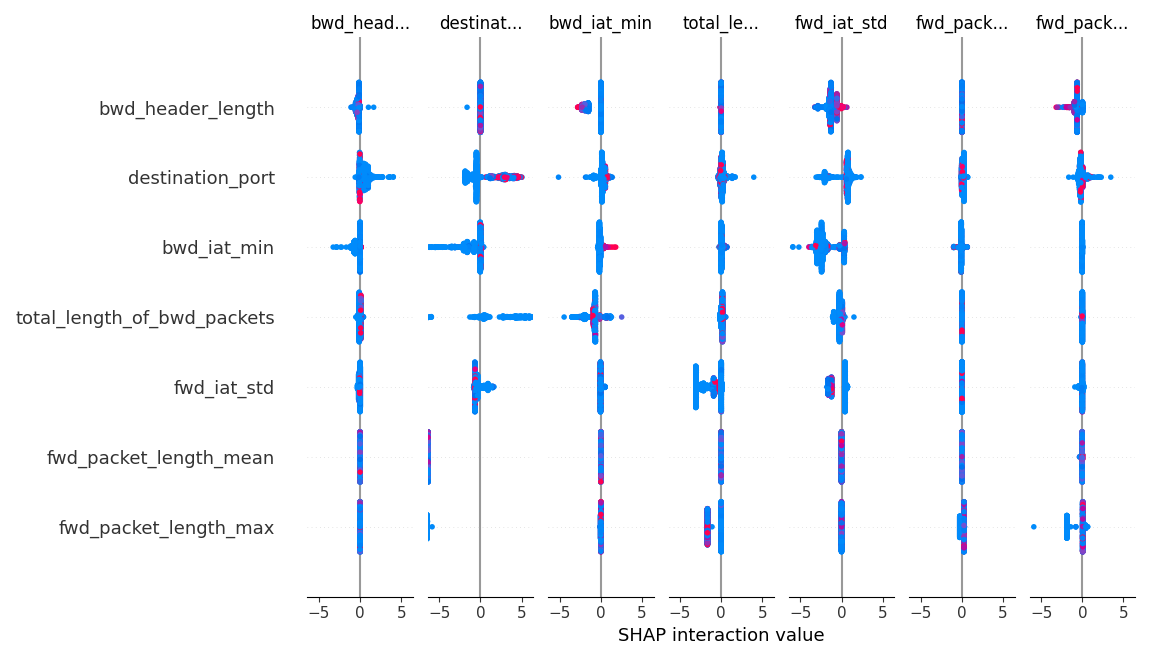
\includegraphics[width=0.7\linewidth]{assets/figures/results/shap_summary_plot_overall.png}
    \caption{SHAP Summary Plot}
\end{figure}
\end{frame}

% Slide 9: Comparative Analysis
\begin{frame}{Comparative Analysis}
\begin{itemize}
    \item XGBoost vs RF, LightGBM, CatBoost.
    \item Outperforms competitors in F1-Macro and Accuracy.
    \item Demonstrates efficiency-accuracy tradeoff for NIDS deployment.
\end{itemize}
\begin{figure}
    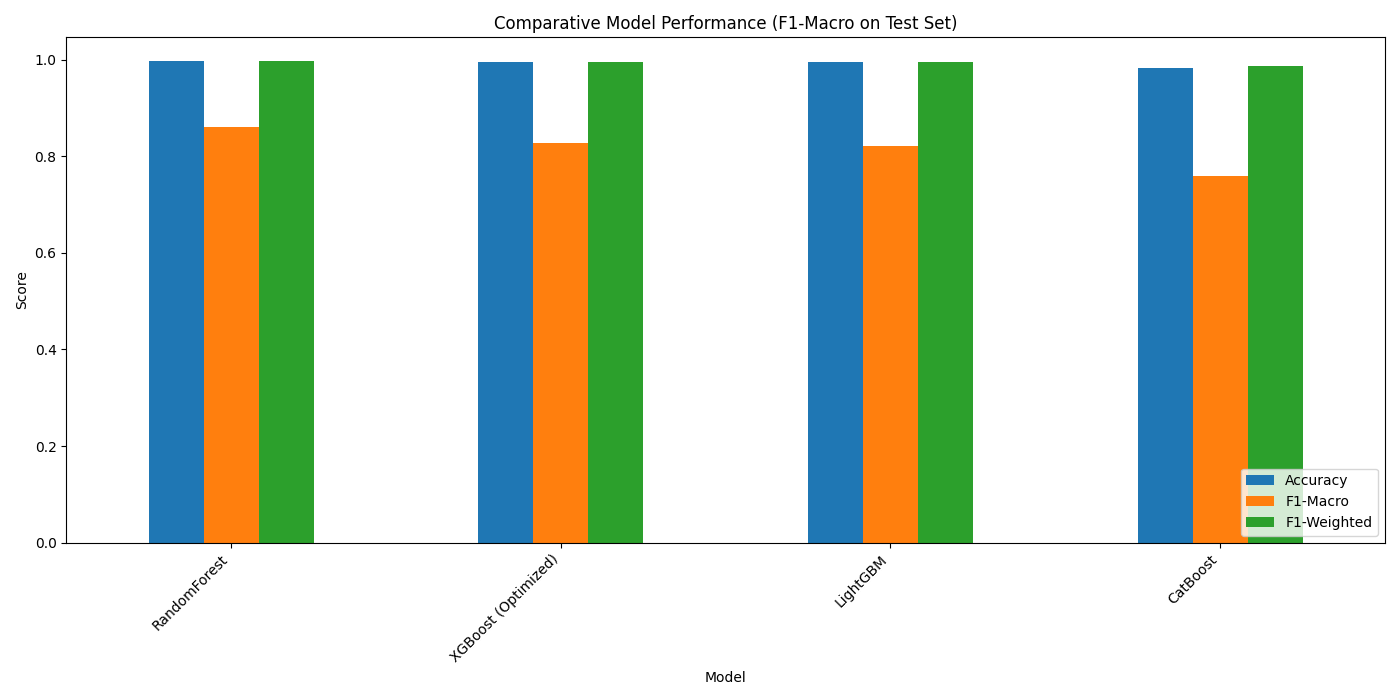
\includegraphics[width=0.7\linewidth]{assets/figures/results/comparative_performance_summary.png}
    \caption{Comparative Performance Summary}
\end{figure}
\end{frame}

% Slide 10: Research Insights
\begin{frame}{Key Insights}
\begin{itemize}
    \item Classical ML is viable for computationally constrained NIDS.
    \item Class imbalance handling is critical for rare attack detection.
    \item Pipeline combines pre-processing, feature selection, tuning, and evaluation effectively.
\end{itemize}
\end{frame}

% Slide 11: Limitations and Future Work
\begin{frame}{Limitations and Future Work}
\begin{itemize}
    \item Dataset limitations: generalization to unseen attacks.
    \item Feature set: only CICFlowMeter features used.
    \item Future directions:
    \begin{itemize}
        \item Test on other datasets (CSE-CIC-IDS2018, UNSW-NB15, IoT)
        \item Hybrid models combining classical ML + deep learning
        \item Real-time deployment and adversarial robustness
        \item Explainable AI for operational decision support
    \end{itemize}
\end{itemize}
\end{frame}

% Slide 12: Conclusion
\begin{frame}{Conclusion}
\begin{itemize}
    \item XGBoost effectively detects multi-class network intrusions on CIC-IDS2017.
    \item SMOTETomek class balancing ensures performance on rare attack types.
    \item Provides an end-to-end pipeline for NIDS: preprocessing, modeling, tuning, and evaluation.
    \item Classical ML offers a practical, computationally efficient solution compared to deep learning.
\end{itemize}
\end{frame}

\frame{\titlepage}

\end{document}

